Over the past years, soft robotics have been a growing field of interest, as they have the potential to safely perform complex tasks in a human-centred environment. Besides executing tasks safely, the robot is demanded to be robust. Safety and robustness can be combined in the robotics design by considering material properties, locomotion, and morphology found in living organisms. Examples of bio-inspired soft robots include emulated trunks \cite{hannan2003kinematics} inspired by the proboscis of an elephant (Figure \ref{fig:BHA}), robots based on the arm of octopus \cite{wang2013visual}, or robots that replicate the movement of fish \cite{marchese2014autonomous}. These robots are created from soft and flexible materials, which ensures safe interaction with humans. However, they do have the necessary properties to grasp and pick-up objects. This flexibility theoretically gives the robot an infinite amount of degrees-of-freedom (DOFs). The robots redundancy gives rise to some advantages and challenges. One major advantage is, that a soft robot can exploit its redundancy to reach an end-effector position in multiple ways. Additionally, it enables the robot to grasp objects around obstacles more easily compared to rigid robots. Nevertheless, its theoretical infinite DOFs makes controlling these robotic systems more challenging as the robot is highly under-actuated. 




\begin{figure}[H]
    \centering
    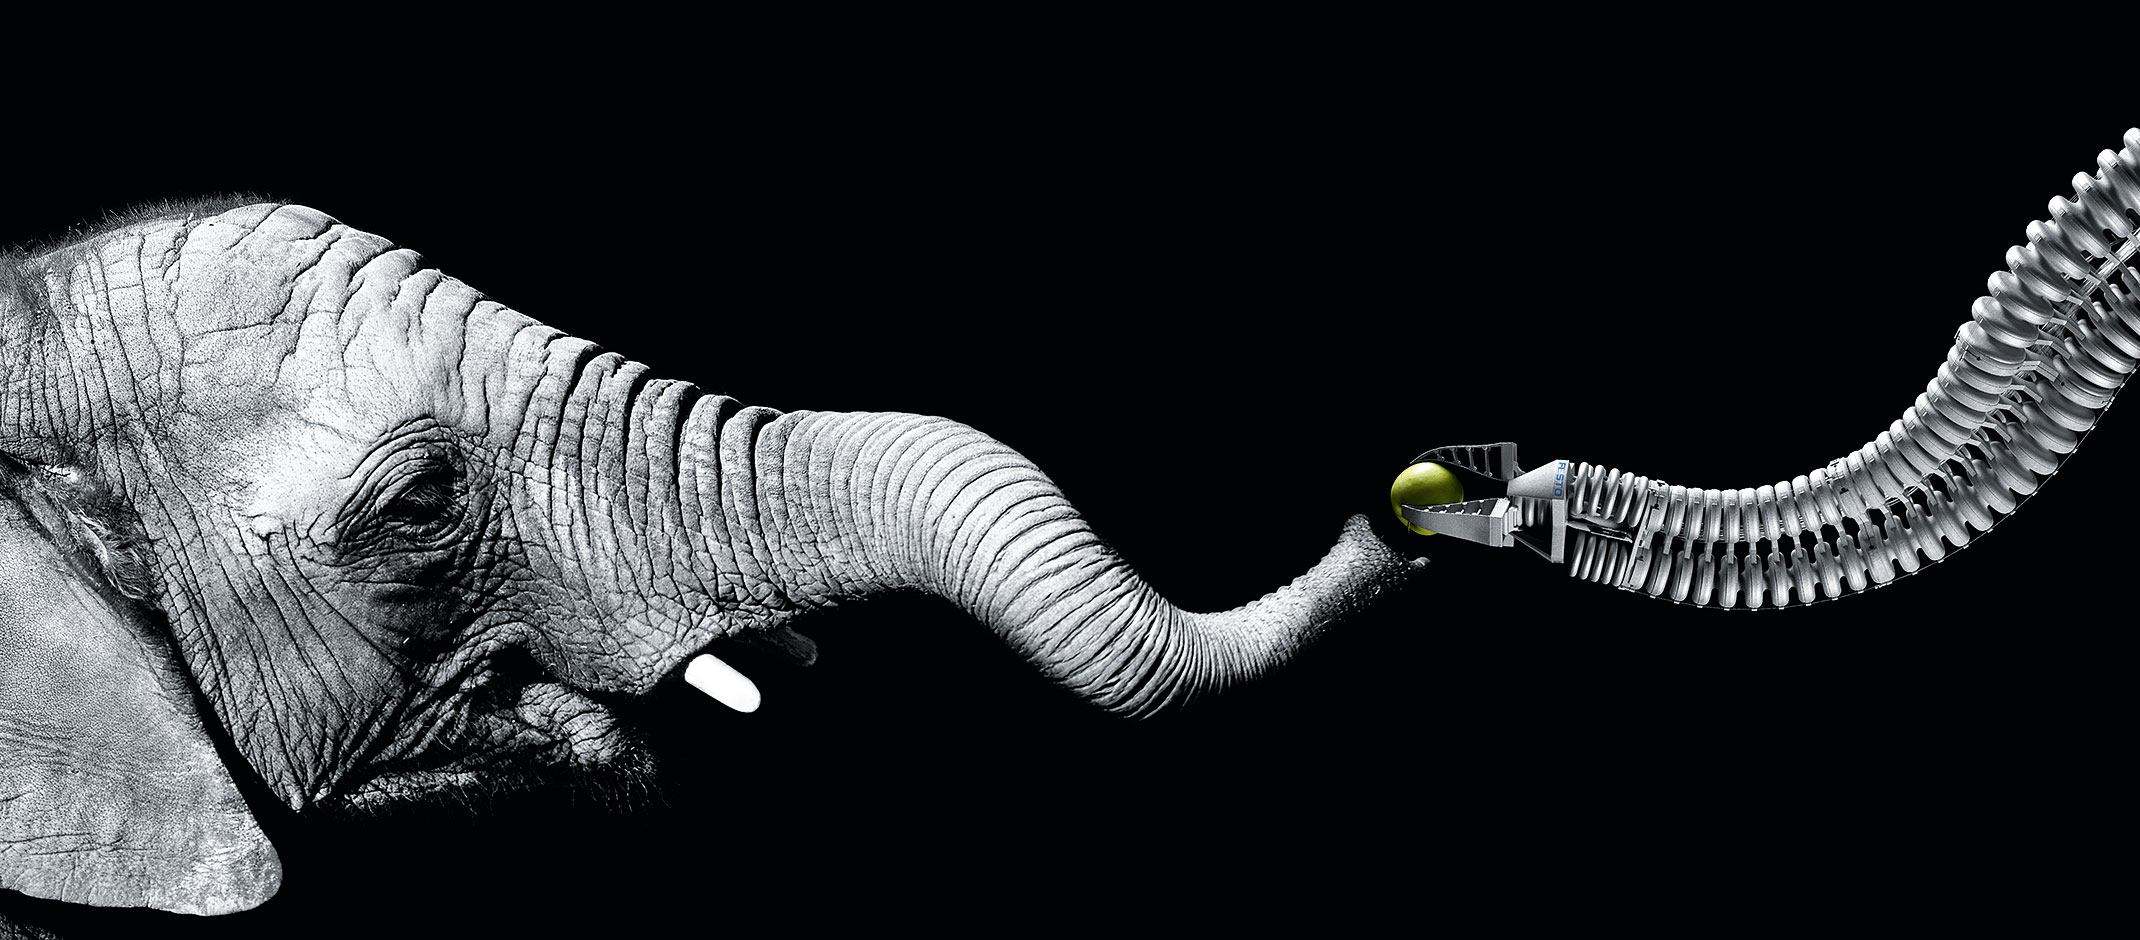
\includegraphics[width = \textwidth]{Figures/BHAelephant.jpg}
    \caption{Bionic Handling Assistant inspired by the trunk of an elephant \cite{BHA}.}
    \label{fig:BHA}
\end{figure}

  \begin{minipage}{\linewidth}
      \centering
      \begin{minipage}{0.44\linewidth}
          \begin{figure}[H]
              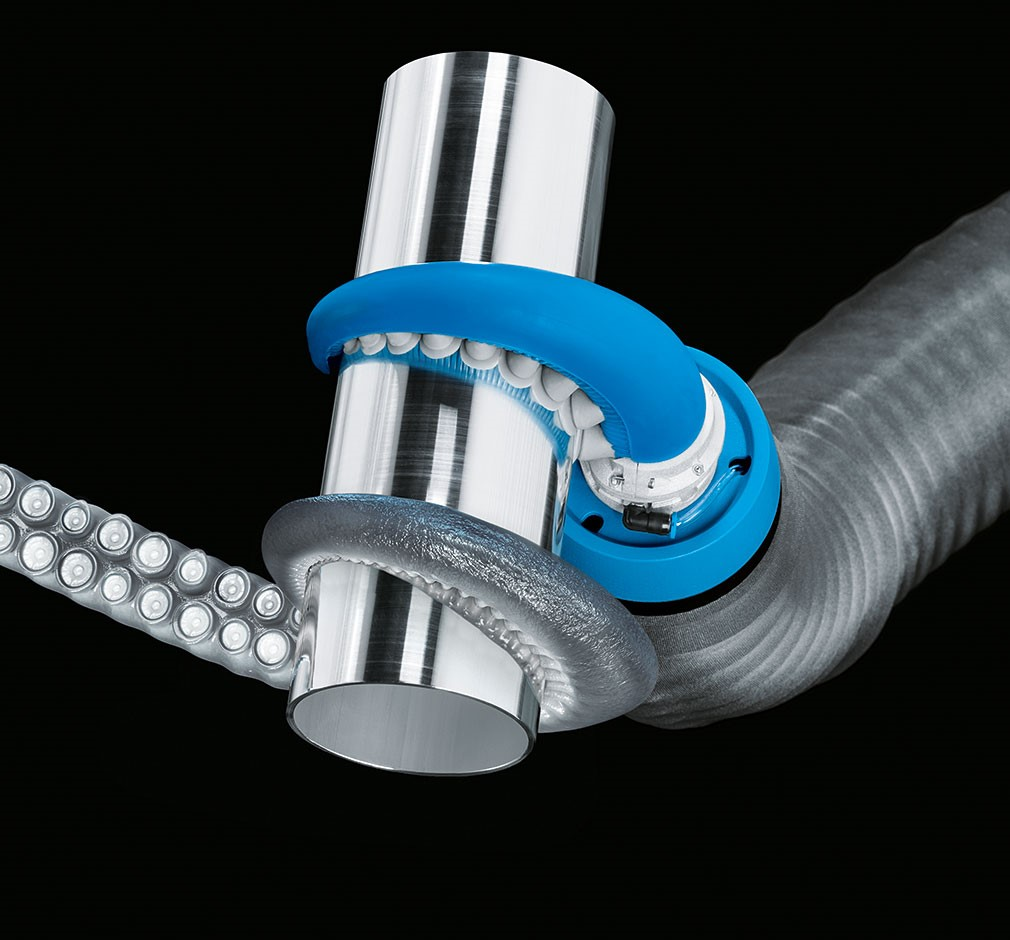
\includegraphics[width=\linewidth]{Figures/tentaclegripper (2).jpg}
              \caption{Octopus-inspired robot able to move and manipulate a wide range of objects \cite{octopus}.}
          \end{figure}
      \end{minipage}
      \hspace{0.05\linewidth}
      \begin{minipage}{0.44\linewidth}
          \begin{figure}[H]
              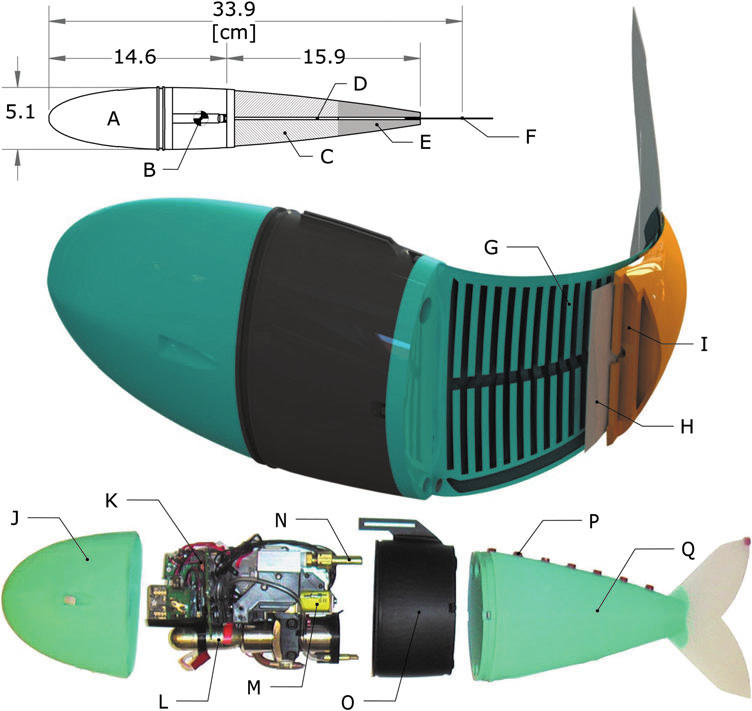
\includegraphics[width=\linewidth]{Figures/fish.jpg}
              \caption{Bio-inspired soft robot replicating movement of a fish \cite{marchese2014autonomous}.}
          \end{figure}
      \end{minipage}
  \end{minipage}



The major difference between soft robots and the well-known rigid robots is the robots' compliance \cite{trivedi2008soft}. Rigid robots generally consist of multiple rigid links that have mechanical actuators inside the joints. Each of this joint controls an additional DOF. A mechanical system is considered redundant if it has more degrees of freedom than those strictly required to execute a given task \cite{chiaverini2016redundant}. Opposed to rigid robots, bio-inspired robots do not necessarily have these links, and are therefore called continuum robots. Due to there continuous morphology, these robots are inherently redundant. Bio-inspired continuum robots can generally be classified into two categories namely, hard continuum robots and soft continuum robots. In general, hard continuum robots consist of rigidly linked vertebrates that form the backbone of the soft robot. This backbone is compliant resulting in a smooth deformation of the robot when external load is applied. An example is the elephant trunk's robot \cite{cieslak1999elephant}, which consists of eight elastic segments linked together by coil springs. Each segment has two pairs of strings that can control the movement of each individual segment. Servo or linear actuators can be use to wind and unwind the strings with that controlling the movement of the robot, these are so called tendon-driven robots. Soft continuum robots are commonly composed of materials, whose mechanical strength is close to those of biological materials such as, muscles, skin, cartilage, and have a Young's modulus of around 1 gigapascal \cite{rus2015design}. Soft robots are generally pneumatically actuated, an example is the Bionic Handling Assistant (BHA) \cite{rolf2012constant} as shown in Figure \ref{fig:BHA}. By inflating chambers this robot is able to extend and bend. Soft robots are commonly highly dexterous, enabling them grasp objects around obstacles. There are multiple challenges with regards to controlling soft robots. Due to its inherently flexible nature, heavy loads at the end-effector can cause deformation throughout the whole mechanical structure of the robot. Furthermore, the distributed body mass of the robot can have similar effects. This makes position sensing more difficult compared to a rigid manipulator, where forward kinematics can be easily formulated. Additionally, due to hyper-flexibility, multiple positions with the same end-effector position are possible, making the robot configuration for a given end-effector position non-unique. 
